\documentclass[11pt]{book}

\usepackage{fontspec}
\setmainfont{TeX Gyre Pagella}
\usepackage[margin=1.25in]{geometry}
\usepackage{titlesec}
\usepackage[colorlinks=true,linkcolor=black,citecolor=black,urlcolor=black]{hyperref}
\usepackage{csquotes}
\usepackage{tikz}

\titleformat{\chapter}[display]{\normalfont\huge\bfseries}{Chapter \thechapter}{20pt}{\Huge}
\titleformat{\section}{\normalfont\Large\bfseries}{\thesection}{1em}{}
\titleformat{\subsection}{\normalfont\large\bfseries}{\thesubsection}{1em}{}

\title{\textbf{Fusion Without Recovery}\\[0.3em]
\large Genome Architecture as Distinction Holonomy\\[0.3em]
\normalsize An Interpretive Reading of Topological Mixing in Animal Chromosome Evolution}
\author{Flyxion \\ \textit{Independent Researcher}}
\date{2026}

\begin{document}

\frontmatter
\maketitle

\chapter*{Abstract}
\noindent Schultz, Bl\"umel, Destanovi\'c, Sarigol, and Simakov (2026) show that chromosome fusion in animal genomes, once followed by intrachromosomal mixing, is statistically irreversible: a later fission event may restore the ancestral chromosome count without restoring the ancestral partition of loci. This book treats that result as fixed and asks a narrower question, developed here at full length rather than in a single essay's compass. Does the mismatch between a coarse structural recurrence and a fine-grained historical non-recovery admit a precise redescription in the vocabulary of distinction holonomy, in which a loop closed at one level of observation fails to close at a finer level of transported structure? The book argues that it does, and that the resulting redescription clarifies, without extending, the empirical paper's own claims. It introduces no new biological mechanism, and it separates carefully, and at each stage, what Schultz et al. establish from what a subsequent conservation-policy reading of their work asserts without direct support in the paper itself.

\tableofcontents
\listoffigures

\mainmatter

\chapter{Introduction}

A chromosome count is a small piece of information. It is also, on its own, a misleading one. Two genomes with the same number of chromosomes can differ profoundly in how the genetic material within those chromosomes is organized, and a single lineage can pass through a fusion event, an extended period of intrachromosomal mixing, and a later fission event, arriving at a chromosome count identical to the one it started with while carrying an internal organization that bears no simple relationship to its ancestral state. Schultz, Bl\"umel, Destanovi\'c, Sarigol, and Simakov's 2026 study of animal chromosome evolution documents this pattern across a large comparative dataset and gives it a precise name: statistical irreversibility. The count can return. The partition of loci that the count was standing in for, at the moment of fusion, generally does not.

This book is an extended, chaptered treatment of a single interpretive question raised by that result. The question is not biological. It does not propose a new mechanism of chromosome rearrangement, does not challenge the paper's methodology, and does not extend its empirical claims beyond what the paper itself supports. The question is instead about vocabulary: given a well-established mismatch between a coarse observable that appears to complete a loop and a finer structure that does not, is there a precise, non-metaphorical way to describe that mismatch, and does describing it that way clarify anything the biology alone leaves implicit?

The candidate vocabulary is distinction holonomy, developed elsewhere as a general framework for describing situations in which a system's coarse-grained trajectory closes while a finer-grained structure transported alongside it fails to return to its starting configuration. The framework did not originate with genome evolution and was not built with genome evolution in mind. Its application here is a test of whether a formal apparatus developed for other cases, ranging from repair and continuation in computational and physical systems to broader questions about persistence under transformation, supplies genuine descriptive traction on a biological result it had no hand in producing. That test can fail. Part of this book's task, developed at length in later chapters rather than compressed into a closing caveat, is to be honest about where the vocabulary adds precision and where it adds nothing beyond restating what the biology already says more plainly.

Three commitments organize everything that follows and are stated here so that they can be checked against every subsequent chapter rather than taken on faith.

The first commitment is that the empirical paper's findings are treated as fixed. This book does not evaluate Schultz et al.'s methodology, does not propose alternative explanations for their results, and does not attempt to adjudicate the open questions the paper itself leaves open, such as whether regulatory entanglement generally explains long-term architectural persistence. Where the paper is uncertain, this book remains uncertain alongside it. Chapter 3 is devoted entirely to stating, as precisely as possible, the boundary between what the paper establishes and what it does not, and that boundary is placed early, before any interpretive material is introduced, specifically so that later chapters cannot quietly borrow certainty they have not earned.

The second commitment is that the interpretive vocabulary introduced in Chapters 4 and 5 is presented as an interpretation, not as a discovery about the underlying biology. Chapter 4 builds the coarse-versus-fine state space distinction slowly and abstractly, using a worked non-biological example before the genome architecture case is introduced, so that the reader can evaluate the formal structure on its own terms before seeing it applied. Chapter 5 then develops the fuller holonomy vocabulary and states explicitly which parts of that vocabulary are being used in a restricted, illustrative sense and which parts are not being invoked at all.

The third commitment is that a structural claim about a genome and an evidentiary claim about what scientists can know from that genome are kept distinct throughout. A genome's present organization constrains which further transformations are reachable from it regardless of whether anyone examines that genome, and this causal fact requires no observer. Turning that constraint into a claim about a specific ancestral fusion event, at a specific point in a phylogeny, requires an inferential method, and Evolutionary Genome Topology, a central component of the comparative and phylogenetic apparatus Schultz et al. built for this purpose, is the method that does much of that work in the present case. Chapters 6 and 7 develop this distinction in detail, using it to sharpen rather than complicate the sense in which a genome can be said to preserve its own history.

The chapters that follow proceed roughly in the order these three commitments suggest. Chapter 2 lays out the biology in more depth than the original essay allowed, including a careful separation of the two layers of irreversibility the paper identifies. Chapter 3 states the limitations. Chapters 4 and 5 build the interpretive vocabulary from the ground up. Chapters 6 and 7 develop the relationship between structural constraint and evidentiary status. Chapter 8 states plainly what the interpretive layer does not add. Chapter 9 closes with a formulation intended to survive contact with a reader who has read only that final chapter and wants to know, in a few sentences, what the book actually claims.

\chapter{The Biology of Statistical Irreversibility}

\section{Two Kinds of Fusion}

Chromosome fusion is not a single event type. A fusion in which two chromosomes join and no subsequent rearrangement disturbs the boundary between their formerly separate gene complements is, in principle, a reversible event: the genetic material needed to reconstruct the ancestral partition remains intact, organized in two contiguous, undisturbed blocks, and a fission event that respects the original boundary would restore the ancestral state exactly. Fusions of this kind are not the subject of Schultz et al.'s irreversibility claim, and distinguishing them from the second kind is necessary before the claim can be stated correctly.

The second kind of fusion is followed, over evolutionary time, by intrachromosomal rearrangement: inversions, translocations, and other mechanisms that relocate genetic material within the fused chromosome. As these rearrangements accumulate, genes that originated on the two ancestral chromosomes become progressively interleaved along the fused chromosome's length. It is this second process, fusion followed by mixing, that the paper identifies as statistically irreversible, and the qualifier statistical is doing real work in that phrase. The claim is not that some biochemical mechanism specifically forbids a fission event from ever recreating the ancestral partition. Fission mechanisms operate on chromosomes as they presently exist; they do not have access to, and are not constrained by, the ancestral arrangement that preceded mixing. Given a sufficiently interleaved chromosome, the number of possible fission points and subsequent rearrangement paths that would need to be traversed to reconstruct the original two-chromosome partition, out of the vastly larger number of paths available to ordinary undirected rearrangement processes, becomes small enough to be effectively unreachable. Irreversibility here describes the shape of a probability distribution over evolutionary trajectories, not a prohibition written into the mechanics of any single rearrangement event.

\begin{figure}[h]
\centering
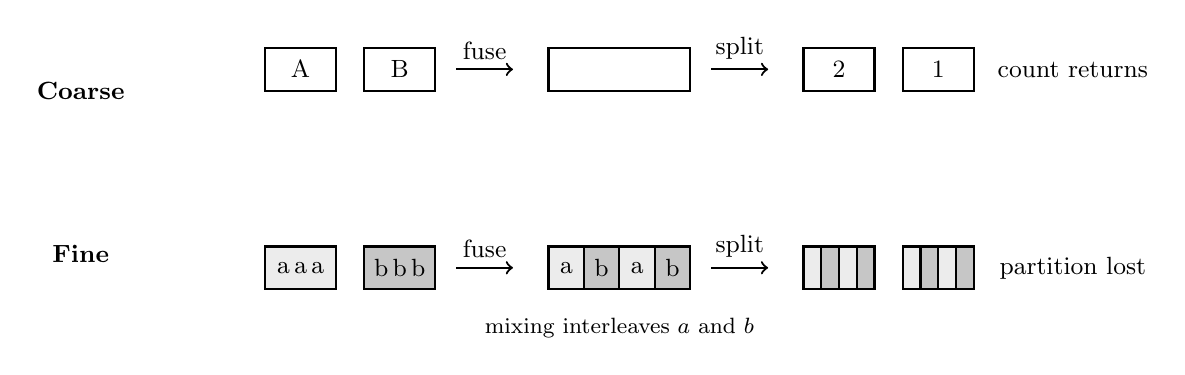
\begin{tikzpicture}[scale=0.9, every node/.style={font=\small}]
  % Coarse row
  \node at (-2.6,3.0) {\textbf{Coarse}};
  \draw[thick] (0,3) rectangle (1,3.6) node[midway]{A};
  \draw[thick] (1.4,3) rectangle (2.4,3.6) node[midway]{B};
  \draw[->,thick] (2.7,3.3) -- (3.5,3.3) node[midway,above]{fuse};
  \draw[thick] (4,3) rectangle (6,3.6);
  \draw[->,thick] (6.3,3.3) -- (7.1,3.3) node[midway,above]{split};
  \draw[thick] (7.6,3) rectangle (8.6,3.6) node[midway]{2};
  \draw[thick] (9.0,3) rectangle (10.0,3.6) node[midway]{1};
  \node at (11.4,3.3) {count returns};

  % Fine row
  \node at (-2.6,0.7) {\textbf{Fine}};
  \draw[thick,fill=gray!15] (0,0.2) rectangle (1,0.8) node[midway]{a\,a\,a};
  \draw[thick,fill=gray!45] (1.4,0.2) rectangle (2.4,0.8) node[midway]{b\,b\,b};
  \draw[->,thick] (2.7,0.5) -- (3.5,0.5) node[midway,above]{fuse};
  \draw[thick,fill=gray!15] (4,0.2) rectangle (4.5,0.8) node[midway]{a};
  \draw[thick,fill=gray!45] (4.5,0.2) rectangle (5.0,0.8) node[midway]{b};
  \draw[thick,fill=gray!15] (5.0,0.2) rectangle (5.5,0.8) node[midway]{a};
  \draw[thick,fill=gray!45] (5.5,0.2) rectangle (6.0,0.8) node[midway]{b};
  \node at (5,-0.35) {\footnotesize mixing interleaves $a$ and $b$};
  \draw[->,thick] (6.3,0.5) -- (7.1,0.5) node[midway,above]{split};
  \draw[thick,fill=gray!15] (7.6,0.2) rectangle (7.85,0.8);
  \draw[thick,fill=gray!45] (7.85,0.2) rectangle (8.1,0.8);
  \draw[thick,fill=gray!15] (8.1,0.2) rectangle (8.35,0.8);
  \draw[thick,fill=gray!45] (8.35,0.2) rectangle (8.6,0.8);
  \draw[thick,fill=gray!15] (9.0,0.2) rectangle (9.25,0.8);
  \draw[thick,fill=gray!45] (9.25,0.2) rectangle (9.5,0.8);
  \draw[thick,fill=gray!15] (9.5,0.2) rectangle (9.75,0.8);
  \draw[thick,fill=gray!45] (9.75,0.2) rectangle (10.0,0.8);
  \node at (11.4,0.5) {partition lost};
\end{tikzpicture}
\caption{Coarse recurrence alongside fine-grained non-recovery. The coarse chromosome count returns to its starting value (top row), while the fine-grained assignment of loci to ancestral linkage groups $a$ and $b$ does not recover its starting partition once intrachromosomal mixing has interleaved them (bottom row). Shading distinguishes loci originating on the two ancestral chromosomes; the final split's two resulting chromosomes each contain a mixture of both.}
\label{fig:coarse-fine-mismatch}
\end{figure}

\section{Two Layers of the Irreversibility Claim}

Schultz et al.'s account separates into two layers that are frequently run together in informal summaries of the work and that this book keeps apart throughout.

The first layer is the loss of ancestral partition information through mixing entropy. This layer is the paper's best-supported claim. It follows directly from treating rearrangement as a process that increases positional entropy among orthologous loci, and the paper's own methodology, comparing ortholog positions across many genomes and reconstructing ancestral linkage groups from that comparison, is built specifically to measure it. As mixing accumulates, the amount of information available, in the present genome, about which locus originated on which ancestral chromosome decreases, and this decrease is measurable directly from the comparative dataset without invoking any claim about why particular arrangements persist rather than others.

The second layer is regulatory entanglement: the hypothesis that some mixed arrangements persist not merely because nothing has yet disrupted them, but because new regulatory relationships, such as shared control by a transcription factor, have formed between loci that mixing brought into proximity, so that disrupting the arrangement would now carry a fitness cost. Loci encoding structural proteins, the collagen peptides among the more familiar examples, illustrate the general kind of gene for which such newly formed regulatory proximity might plausibly matter, though nothing in what follows depends on collagen loci specifically, and the paper makes no claim about any particular gene family in this connection. This layer is considerably weaker, and the paper is explicit about its own evidentiary limits here. The evidence offered is comparative persistence, certain locus pairings recur across clades and survive for very long evolutionary timescales, together with suggestive transcription-factor-binding data consistent with functional coupling. Neither of these observations, individually or together, rules out a simpler explanation: that these arrangements persist neutrally, because no subsequent rearrangement event happened to disrupt them, and their long persistence reflects the frequency of disruptive rearrangement events rather than any selective pressure protecting the arrangement itself. The paper identifies functional validation, presumably through direct perturbation of the regulatory relationships in question, as necessary future work, and does not claim to have already distinguished the entanglement hypothesis from the neutral-persistence alternative.

Keeping these two layers separate matters for everything that follows in this book. The interpretive material developed in later chapters draws primarily on the first, well-supported layer. Where the second, more speculative layer becomes relevant, later chapters flag it explicitly rather than allowing the interpretive vocabulary to inherit a level of confidence the underlying biology does not yet warrant.

\section{Evolutionary Genome Topology}

The comparative method underlying both layers of the irreversibility claim is Evolutionary Genome Topology, the analytical framework Schultz et al. developed for this study, which they implement in two complementary forms. The first, MGT, compares individual genomes directly: for a given genome, it builds a matrix of pairwise ortholog distances, treating that genome, or haplotype, as a single sample. The second, MLT, compares loci rather than genomes: for a given orthologous locus or locus neighborhood, it averages that locus's pairwise distances to others across many species, with the averaging weighted by phylogenetic relationships among the sampled taxa so that heavily sampled clades do not dominate the result. Both representations can then be projected into a lower-dimensional space using manifold-learning techniques, principally UMAP, producing a visualizable ``architecture space'' in which genomes, under MGT, or loci, under MLT, with similar positional structure appear near one another and those with divergent structure appear far apart.

Each choice underlying either implementation, the distance metric, the phylogenetic weighting in MLT, the dimensionality-reduction algorithm applied afterward, is a specific, inspectable analytical decision, and the resulting representation is constructed by those decisions rather than an independent object discovered by them. This distinction becomes important in Chapter 3, where the status of the resulting ``architecture space'' as an analytical artifact, rather than as direct evidence of an underlying biological manifold, is addressed at length. For the purposes of this chapter, the relevant point is narrower: the method, in either form, is powerful enough to detect the pattern this book is interested in, the recurrence of a coarse observable, chromosome count, alongside the non-recurrence of a finer observable, ancestral locus partition, and it detects that pattern directly, through positional distance measurements, rather than through any assumption about holonomy, gauge structure, or the interpretive vocabulary introduced in Chapters 4 and 5.

\section{The 406/406 Result, Stated Carefully}

Among the paper's findings, one result is both its most striking and its most frequently overstated in secondary discussion, and it is worth isolating here before any interpretive weight is placed on it. Schultz et al. report that all 406 pairwise combinations among 29 reconstructed ancestral linkage groups occur somewhere in their sampled animal genomes. Meanwhile, the space of possible internal gene arrangements, the ways in which the contents of two fused ancestral linkage groups can subsequently be interleaved, remains comparatively sparsely sampled across the same dataset.

The temptation, visible in some secondary reporting of this result, is to read it as showing that combination is broadly reachable while internal mixing is specifically restricted, as though evolution freely explores which chromosomes fuse but is somehow constrained in how their contents subsequently mix. This reading outruns what sparse sampling can establish. A combinatorial space of internal arrangements is vastly larger than a combinatorial space of pairwise chromosome combinations, and sparse coverage of a much larger space, relative to near-complete coverage of a much smaller one, is exactly what would be expected even if no differential restriction on reachability existed at all. Sparse coverage is additionally consistent with several distinct explanations that the paper's data does not distinguish between: some regions of arrangement space may simply be too large to have been visited by any finite sample of genomes regardless of any restriction; some arrangements may be young, having arisen too recently in evolutionary time for their descendant lineages to have been sampled; some may have been reached and then selected against; and some may be inaccessible through the ordinary rearrangement mechanisms available to a given lineage's biology. The paper does not adjudicate between these possibilities, and this book does not attempt to on its behalf.

The formulation that the evidence actually supports, and the one used throughout the remainder of this book, is narrower and still substantial: pairwise fusion space appears saturated at the sampled scale, while internal configuration space is far from saturated by the same measure. This is a fact about sampling density relative to space size, established directly by the comparative dataset, and it should not be asked to carry a stronger claim about differential reachability that the data alone cannot support.

\chapter{What the Evidence Does and Does Not Show}

This chapter is placed before any interpretive material for a specific reason. Everything from Chapter 4 onward redescribes a result already established by Schultz et al., and a redescription can only be as trustworthy as the boundary drawn around what it is redescribing. If that boundary is drawn loosely, the interpretive vocabulary risks absorbing claims the empirical paper never made and presenting them back with an unearned appearance of rigor. This chapter draws the boundary carefully, in three parts, before any such vocabulary is introduced.

\section{Regulatory Entanglement Remains a Hypothesis}

The paper's account of why certain mixed genome architectures persist across very long evolutionary timescales rests, for its strongest form, on the regulatory entanglement hypothesis introduced in Chapter 2. It is worth restating, at this point in the book, exactly how much evidentiary weight that hypothesis currently carries, because the temptation to treat it as an established mechanism grows stronger once it becomes attached to a more general vocabulary of persistence and constraint.

The evidence in the paper's favor is comparative persistence and suggestive transcription-factor-binding data. Comparative persistence, a locus pairing recurring and surviving across many millions of years in a clade, is consistent with the arrangement being functionally protected by selection. It is equally consistent with the arrangement simply not having been disrupted, since disruption requires a further rearrangement event, and such events do not occur at a fixed rate independent of chromosomal context. Distinguishing functional protection from undisturbed neutrality requires evidence beyond persistence itself, and the transcription-factor-binding data the paper reports is suggestive rather than dispositive: binding data indicates that a regulatory relationship is structurally possible given the current arrangement, not that the arrangement's persistence is causally explained by that relationship having conferred a selective advantage. The paper states this limitation itself, identifying functional validation, of the kind that would come from directly perturbing the regulatory relationship and observing a fitness consequence, as necessary future work rather than as work already completed.

Nothing in this book depends on regulatory entanglement being true. The interpretive material in later chapters draws on the first, entropy-based layer of irreversibility, which does not require any claim about why particular arrangements persist, only that ancestral partition information degrades as mixing accumulates. Where regulatory entanglement is mentioned again in this book, it is mentioned as an open question the biology has not yet settled, not as a premise the interpretive vocabulary is entitled to assume.

\section{The Architecture Space Is a Constructed Representation}

Evolutionary Genome Topology's ``architecture space,'' introduced in Chapter 2, is the output of a specific analytical construction: ortholog-position distance matrices, built per-genome under MGT or per-locus and phylogenetically weighted under MLT, followed by manifold-learning projection via UMAP. Each of these choices is defensible and the paper documents them clearly, but the resulting space is, for that reason, a representation constructed by a particular method rather than an independently existing object that the method merely discovers. Descriptive language built on top of this representation, trajectories through the space, clustered or isolated regions, persistent pathways, describes patterns visible in this particular embedding. It does not, on its own, establish that evolution is constrained to move along a uniquely defined geometric structure that would exist under some different choice of distance metric, weighting scheme, or dimensionality-reduction algorithm.

This qualification matters for the interpretive chapters that follow, because the temptation in redescribing this result using a geometric vocabulary, connections, curvature, transported structure, is to treat the geometry as though it were already latent in the biology, waiting to be found, rather than as a representation chosen to make certain relationships visible. Chapter 5 addresses this directly by specifying, in advance, which parts of the holonomy vocabulary are being used descriptively, to characterize a pattern the data supports independent of any particular embedding, and which parts would require a stronger claim about an underlying geometric object that this book does not make.

\section{The Conservation Claim Is Not in the Paper}

The most consequential gap between what Schultz et al. establish and what has circulated about their work concerns conservation policy. Secondary reporting on this study, including coverage originating from the researchers' home institution, has suggested that architecturally isolated clades, lineages occupying distinctive regions of the architecture space, might warrant elevated conservation priority on the strength of their genome-topological distinctiveness.

This claim does not appear, in any tested or argued form, in the paper's own conclusions. The paper's conclusion discusses future evolutionary trajectories, speciation dynamics, regulatory novelty, and the value of expanding genome sampling to further taxa. It does not propose, test, or defend a method for translating architectural isolation into a conservation-priority metric, does not compare such a metric against existing measures of evolutionary distinctiveness already used in conservation biology, and does not address the further question of whether genome-topological uniqueness bears any established relationship to ecological importance, functional distinctiveness, or extinction risk, all of which are independent considerations that a conservation-priority argument would need to engage.

None of this means the underlying idea is unreasonable as a direction for future research. Genome-topological isolation is one plausible measure of evolutionary distinctiveness among several that conservation biology already uses, and it is not unreasonable to ask whether it correlates with, or adds information beyond, those existing measures. But that is a further research question, requiring its own argument and its own evidence, not a result this paper has already established. Treating the conservation claim as though it followed directly from the topology, rather than as a plausible but currently unsupported extension of it, is exactly the kind of overreach this chapter exists to prevent from being carried, unexamined, into the interpretive chapters that follow.

\section{The Boundary Stated Plainly}

Three claims, and only three, are treated as the empirical premises of this book: that fusion followed by intrachromosomal mixing progressively erases recoverable ancestral partition information; that this erosion is measurable directly, through Evolutionary Genome Topology's comparative methodology, independent of any claim about why particular resulting arrangements persist; and that pairwise fusion space appears saturated at the sampled scale while internal configuration space does not. Everything else, the causal role of regulatory entanglement, the status of the architecture space as a literal biological manifold, and any relationship between genome topology and conservation priority, remains open, and this book does not close it.

\chapter{Coarse and Fine State Spaces}

\section{A Non-Biological Case, Stated First}

Before applying any interpretive vocabulary to genome architecture, it is worth building the underlying structure in a setting with no biology attached, so that the pattern can be evaluated on its own terms rather than absorbed uncritically alongside the empirical result it will later be used to describe.

Consider a deck of playing cards, arranged initially into two piles of equal size, and consider two different descriptions of the deck's state. The coarse description records only the number of piles: one, or two. The fine description records the full ordering of every card, including which original pile each card came from. Begin with two piles. Merge them into a single pile by an arbitrary interleaving, so that cards from the two original piles are now shuffled together along the single pile's length. Coarsely, this is a fusion: two piles become one. Now split the merged pile into two piles again, at some arbitrary point along its length. Coarsely, this is a fission: one pile becomes two again, and the coarse description, pile count, has returned exactly to its starting value.

The fine description tells a different story. Unless the interleaving performed during the merge happened to place all cards from the first original pile before all cards from the second, an assumption nothing in the merge procedure guarantees and that becomes less and less likely the more thoroughly the cards are shuffled, the new split will not recover the original two piles. Each of the two new piles will generally contain a mixture of cards from both original piles, and no amount of further splitting or merging, performed without reference to a record of which card came from which original pile, can be expected to recover the original partition. The pile count has closed a loop. The assignment of cards to original piles has not.

\begin{figure}[h]
\centering
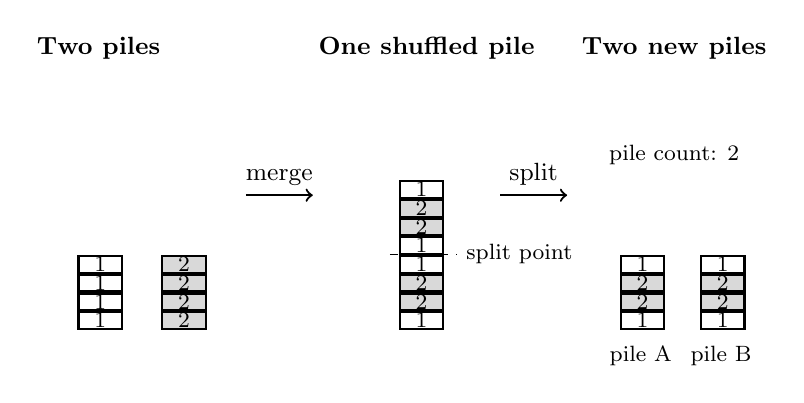
\begin{tikzpicture}[scale=0.85, every node/.style={font=\small}]
  \node at (0,4.2) {\textbf{Two piles}};
  \foreach \i in {0,...,3} { \draw[thick,fill=white] (-0.3,\i*0.28) rectangle (0.35,\i*0.28+0.25) node[midway]{\footnotesize 1}; }
  \foreach \i in {0,...,3} { \draw[thick,fill=gray!30] (0.95,\i*0.28) rectangle (1.6,\i*0.28+0.25) node[midway]{\footnotesize 2}; }

  \draw[->,thick] (2.2,2) -- (3.2,2) node[midway,above]{merge};

  \node at (4.9,4.2) {\textbf{One shuffled pile}};
  \draw[thick,fill=white] (4.5,0) rectangle (5.15,0.25) node[midway]{\footnotesize 1};
  \draw[thick,fill=gray!30] (4.5,0.28) rectangle (5.15,0.53) node[midway]{\footnotesize 2};
  \draw[thick,fill=gray!30] (4.5,0.56) rectangle (5.15,0.81) node[midway]{\footnotesize 2};
  \draw[thick,fill=white] (4.5,0.84) rectangle (5.15,1.09) node[midway]{\footnotesize 1};
  \draw[thick,fill=white] (4.5,1.12) rectangle (5.15,1.37) node[midway]{\footnotesize 1};
  \draw[thick,fill=gray!30] (4.5,1.4) rectangle (5.15,1.65) node[midway]{\footnotesize 2};
  \draw[thick,fill=gray!30] (4.5,1.68) rectangle (5.15,1.93) node[midway]{\footnotesize 2};
  \draw[thick,fill=white] (4.5,1.96) rectangle (5.15,2.21) node[midway]{\footnotesize 1};
  \draw[dashed] (4.35,1.12) -- (5.35,1.12) node[right]{\footnotesize split point};

  \draw[->,thick] (6.0,2) -- (7.0,2) node[midway,above]{split};

  \node at (8.6,4.2) {\textbf{Two new piles}};
  \draw[thick,fill=white] (7.8,0) rectangle (8.45,0.25) node[midway]{\footnotesize 1};
  \draw[thick,fill=gray!30] (7.8,0.28) rectangle (8.45,0.53) node[midway]{\footnotesize 2};
  \draw[thick,fill=gray!30] (7.8,0.56) rectangle (8.45,0.81) node[midway]{\footnotesize 2};
  \draw[thick,fill=white] (7.8,0.84) rectangle (8.45,1.09) node[midway]{\footnotesize 1};
  \node at (8.1,-0.4) {\footnotesize pile A};

  \draw[thick,fill=white] (9.0,0) rectangle (9.65,0.25) node[midway]{\footnotesize 1};
  \draw[thick,fill=gray!30] (9.0,0.28) rectangle (9.65,0.53) node[midway]{\footnotesize 2};
  \draw[thick,fill=gray!30] (9.0,0.56) rectangle (9.65,0.81) node[midway]{\footnotesize 2};
  \draw[thick,fill=white] (9.0,0.84) rectangle (9.65,1.09) node[midway]{\footnotesize 1};
  \node at (9.3,-0.4) {\footnotesize pile B};

  \node at (8.6,2.6) {\footnotesize pile count: 2};
\end{tikzpicture}
\caption{The card-pile example. Two piles (count 2) are merged into one shuffled pile and later split at an arbitrary point back into two piles (count 2 again). Coarsely the loop closes. Neither resulting pile A nor pile B recovers either original pile; both are mixtures of cards labeled 1 and 2.}
\label{fig:card-piles}
\end{figure}

\section{Two Distinct Loops}

This example separates two things that are easy to run together when read quickly: the return of a coarse count, and the closure of a full historical loop. Only the first has occurred. The second has not, and recognizing why it has not requires attending to a specific mechanism: the merge step destroyed information, specifically the mapping from each card's current position to its originating pile, that the split step has no access to and cannot reconstruct.

This mechanism generalizes beyond playing cards. Whenever a system possesses a coarse observable, some low-dimensional summary of its state, and a finer observable, some higher-dimensional structure that the coarse observable summarizes, it is possible for a sequence of transformations to return the coarse observable to its starting value while an intervening step has destroyed the information needed to also return the finer observable to its starting value. The coarse observable's return is not evidence, by itself, that the finer observable has also returned; whether it has depends entirely on whether every step in the sequence preserved enough information to make reconstruction possible.

\section{Applying the Structure to Genome Architecture}

The correspondence to chromosome evolution, established carefully rather than asserted by analogy, is now direct. The coarse observable is chromosome count: the number of distinct chromosomes present in a genome, which fusion decreases by one and fission increases by one. The fine observable is the assignment of individual loci to ancestral linkage groups: which genes originated on which of the ancestral chromosomes that, over evolutionary time, came to be combined into the genome's present configuration.

Fusion followed by fission is, coarsely, a loop: chromosome count decreases and then increases, potentially returning to its starting value. Whether the finer observable, ancestral locus assignment, also returns depends on what happened between the fusion and the fission. If no intrachromosomal mixing occurred during that interval, the ancestral partition remains intact and a fission that respects it would restore the original state exactly, just as an unshuffled merge of two card piles could be split back into the original two piles. If intrachromosomal mixing did occur, and Schultz et al.'s central finding is that it generally does, the mechanism is the same one identified in the card-pile case: the mixing step destroys the positional information a later fission would need in order to recover the ancestral partition, and no subsequent fission mechanism has access to, or is constrained by, information that mixing has already erased.

\section{What This Chapter Has and Has Not Shown}

This chapter has established a general pattern, coarse recurrence without fine recovery, using an example with no biological content, and has then shown that a structurally analogous pattern applies to the fusion-mixing-fission sequence Schultz et al. document. It has not yet introduced the term distinction holonomy, and has deliberately withheld the fuller geometric vocabulary, connections, curvature, transported structure, that Chapter 5 develops. The reason for withholding it here is that the pattern itself, coarse loop closure alongside fine non-recovery, does not require that vocabulary to be stated or understood; the vocabulary, when it is introduced, is a further formalization of this pattern, not a precondition for recognizing that the pattern exists. Readers who find the geometric vocabulary of Chapter 5 unfamiliar or unnecessary can treat this chapter's card-pile example, and its direct application to chromosome architecture, as a complete statement of this book's core observation.

One disanalogy in the card-pile example is worth flagging rather than leaving implicit. A physical card retains its identity through the shuffle: if each card were secretly marked according to its originating pile, or if the initial membership of the two piles had been recorded elsewhere, the ancestral partition would remain fully recoverable from those marks or that record, however thoroughly the deck had been shuffled. What the shuffle destroys is not, strictly, the partition itself, but the partition's recoverability from the deck's own present order considered in isolation from any such record. This distinction, between a fact ceasing to exist and a fact ceasing to be encoded in the particular observable under consideration, matters more than the card example alone can show, and Chapter 7 returns to it directly: whether the genome's ancestral partition is unavailable in the stronger sense or merely unrecovered from the observables Evolutionary Genome Topology examines is exactly the question that chapter's inferential apparatus is built to bear on.

\chapter{Distinction Holonomy: A Formal Vocabulary}

\section{What This Chapter Borrows, and What It Leaves Behind}

Distinction holonomy, as developed at length elsewhere, is a general framework describing persistence, repair, and continuation under transformation, built around a formal apparatus of connections, curvature, and gauge-invariant comparison. That framework was developed to address a wide range of cases, computational, physical, and otherwise, and its full technical machinery is considerably more than the present case requires. This chapter borrows only the minimal part of that vocabulary needed to name, precisely, the pattern established informally in Chapter 4, and states explicitly, at each step, what is and is not being claimed by the borrowing.

\section{Distinctions, Transport, and Loops}

A distinction, in the relevant sense, is any structure finer than the coarse observable under discussion that is nonetheless carried along as the system undergoes a sequence of transformations. In the card-pile example, the coarse observable was pile count, and the distinction was the assignment of each card to its originating pile. In the genome case, the coarse observable is chromosome count, and the distinction is the assignment of each locus to its ancestral linkage group.

A sequence of transformations closes a loop, at the coarse level, when the coarse observable returns to its starting value. Fusion followed by fission closes a loop at the level of chromosome count. The distinction is said to be transported along this loop if each transformation in the sequence carries forward whatever information about the distinction was available going in. Transport can be faithful, preserving the distinction exactly, or lossy, degrading it. An unmixed fusion followed by a boundary-respecting fission transports the locus-assignment distinction faithfully. A mixed fusion followed by an arbitrary fission transports it lossily, and the central empirical fact this book is built around, that intrachromosomal mixing degrades recoverable ancestral partition information, is precisely a statement about lossy transport in this sense.

Holonomy, in the restricted sense used in this chapter, names the mismatch between a loop's closure at the coarse level and the transported distinction's failure to return to its starting configuration along that same loop. Where transport is faithful throughout, the loop closes at both levels and holonomy, in this sense, is trivial: the transported distinction returns along with the coarse observable. Where transport is lossy at some point along the loop, the coarse observable can still return, since coarse closure depends only on the coarse observable's own dynamics, while the transported distinction generally does not, since its return would require the lossy step to have been information-preserving, which by hypothesis it was not.

\begin{figure}[h]
\centering
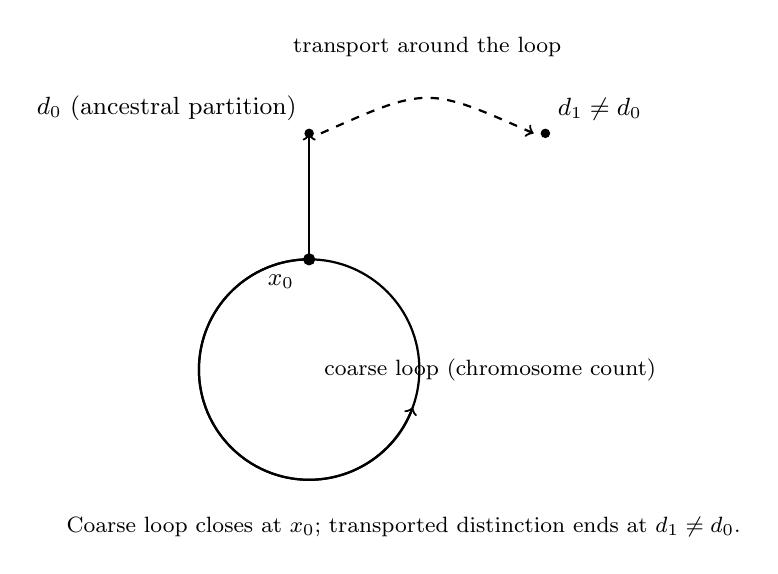
\begin{tikzpicture}[scale=1.0, every node/.style={font=\small}]
  % base loop
  \draw[thick] (0,0) circle (1.4);
  \filldraw (0,1.4) circle (2pt) node[below left=2pt]{$x_0$};
  \draw[->,thick] (0,1.4) arc (90:340:1.4);
  \node at (2.3,0) {\footnotesize coarse loop (chromosome count)};

  % fiber above x0, start
  \draw[->,thick] (0,1.4) -- (0,3.0);
  \filldraw (0,3.0) circle (1.5pt);
  \node[above left=1pt] at (0,3.0) {$d_0$ (ancestral partition)};

  % fiber above x0, end, offset well to the right to show non-return
  \filldraw (3.0,3.0) circle (1.5pt);
  \node[above right=1pt] at (3.0,3.0) {$d_1 \neq d_0$};
  \draw[->,thick,dashed] (0.15,3.0) .. controls (1.5,3.6) and (1.5,3.6) .. (2.85,3.0);
  \node at (1.5,4.1) {\footnotesize transport around the loop};

  \node at (1.2,-2.0) {\footnotesize Coarse loop closes at $x_0$; transported distinction ends at $d_1 \neq d_0$.};
\end{tikzpicture}
\caption{Restricted holonomy, as used in Chapter 5. The coarse observable traces a closed loop back to its starting point $x_0$. The distinction transported alongside it, here ancestral locus assignment, begins at $d_0$ but arrives at a different value $d_1$ after the loop closes, reflecting lossy transport during the mixing step. No connection is formally specified or integrated; the diagram illustrates the mismatch the term names, not a derivation from local transport rules.}
\label{fig:holonomy-loop}
\end{figure}

\section{What Is Not Being Claimed}

Three clarifications bound this chapter's use of the vocabulary, each addressing a stronger claim the language might otherwise be read as making.

First, holonomy in the fuller technical sense developed elsewhere is typically defined relative to a specific connection, a rule specifying how a distinction is transported infinitesimally along any path, from which finite-loop behavior is derived by integration. This chapter does not construct such a connection for the genome case, does not claim that ancestral locus assignment obeys any particular local transport rule beyond ``mixing degrades it and undisturbed regions preserve it,'' and uses holonomy here as a description of the coarse-versus-fine mismatch directly, not as the output of a connection formally specified and integrated. Readers familiar with the fuller framework should read every use of the term in this book as the restricted, descriptive sense defined in this chapter, not the full gauge-theoretic apparatus.

Second, the fuller framework distinguishes curvature, a local property of a connection, from holonomy, a global property measured around a specific loop, and treats the flat-but-multiply-connected case, where local transport is loss-free everywhere but global topology still produces nontrivial holonomy, as a distinct and important possibility. This chapter does not adjudicate whether genome mixing is better described as locally lossy, curvature-like, or as an instance of the flat-but-multiply-connected case; the entropy-based account in Chapter 2 is naturally read as locally lossy, and this book adopts that reading without argument for the more exotic alternative, since nothing in the biology as established requires it.

Third, and most importantly given Chapter 3's caution about the architecture space, none of this chapter's vocabulary depends on treating Evolutionary Genome Topology's UMAP embedding as the geometric space in which holonomy is being measured. The holonomy described here is a property of the relationship between chromosome count and ancestral locus assignment, established directly from Schultz et al.'s comparative and phylogenetic evidence. The architecture space is a separate, later analytical construction, useful for visualizing patterns across many genomes at once, and this chapter's claims would survive entirely if that particular embedding technique were replaced by a different one.

\section{Why the Vocabulary Earns Its Place}

Given these restrictions, what does the vocabulary add beyond the plain statement, already available at the end of Chapter 4, that chromosome count can return while ancestral locus assignment generally does not? The addition is modest but real: it names the general pattern, coarse recurrence alongside lossy fine-grained transport around a loop, in a way that makes it recognizable as an instance of a broader class of phenomena rather than as an isolated biological curiosity. This naming is not required to understand the genome case, which Chapter 4 already made fully intelligible on its own terms, but it does connect this case to others where the same structural mismatch has been identified, including cases entirely outside biology, and that connection is the vocabulary's only claimed contribution.

\chapter{History as Constraint, Not Inscription}

\section{Two Ways an Artifact Can Preserve Its Past}

An artifact can preserve its history in at least two structurally different ways, and distinguishing them precisely is necessary before the genome can be described, without overclaiming, as preserving anything at all.

The first way is propositional. A version-control system such as Git preserves history by recording explicit assertions: a commit object asserts a particular parent, a particular timestamp, and a particular content state, and this assertion persists as an inspectable, addressable object whether or not anyone subsequently reads it. The assertion can be true or false, can be checked against other evidence, and exists as a discrete unit of content, separable in principle from the artifact whose history it describes. A corrupted or falsified commit history is still, in this sense, a history, an assertion that happens to be wrong, rather than an absence of any assertion at all.

The second way is dispositional. A system can preserve its history not by asserting anything about that history, but by having its present organization shaped, in a way that persists, by the transformations it has undergone, such that some subsequent transformations remain reachable from its present state and others do not. Nothing in a dispositionally history-preserving system contains a proposition about what happened to it. What persists is a constraint on what can happen to it next, a constraint that exists whether or not the system, or anything examining the system, represents that constraint explicitly.

\section{The Genome as a Dispositional Case}

The genome, described carefully, is dispositional in exactly this sense, and describing it any other way risks a category error worth spelling out explicitly. No genome contains a proposition asserting that a particular fusion occurred at a particular point in a particular lineage's history. Nothing internal to the genome functions as a commit message, a timestamp, or an explicit record of ancestry in the propositional sense Git exemplifies. What the genome does contain, as a direct consequence of the mixing process documented in Chapter 2, is a present organization of loci that leaves the ancestral partition without any ordinary evolutionary process directed toward recovering it, so that the probability of an undirected sequence of rearrangements landing back on that partition becomes vanishingly small rather than zero. The fusion is preserved not because the ancestral partition has been removed from what is dynamically possible, but because nothing in the genome's present organization or in the rearrangement processes acting on it is oriented toward reconstructing it.

This distinction is not a demotion of the genome's historical content relative to an explicitly recorded history; it is a correction of what kind of historical content is actually present. A dispositional constraint is a genuine causal fact about the system, not a weaker or more metaphorical kind of memory. The mixed genome's present organization really does make certain reconstructions effectively inaccessible, in exactly the way that Chapter 4's shuffled deck of cards really does make recovery of the original two piles effectively inaccessible to any process operating only on the shuffled deck's present order. What is absent, in both cases, is not the causal fact of that inaccessibility but any propositional record, internal to the artifact itself, asserting that it has occurred or explaining why.

\section{No Observer Is Required for the Constraint}

A further distinction, easy to blur once the language of preservation and memory is in play, concerns the role of an observer. The causal constraint a mixed genome imposes on its own future reachable states operates regardless of whether any scientist, or any organism, examines that genome. Two mixed chromosomes remain mixed, and the corresponding ancestral partition remains statistically unrecovered by ordinary undirected processes, whether or not Evolutionary Genome Topology, or any comparable method, is ever applied to detect that fact. The constraint is a property of the genome's material organization and the dynamics available to act on it, not a property that depends on anyone's knowledge of, or attention to, that organization.

This point matters because it separates two questions that a looser treatment of ``the genome remembers its history'' tends to run together: whether the constraint exists, and whether anyone can currently demonstrate that it exists and characterize what it constrains. The first question has a definite answer, established directly by the biology in Chapter 2, independent of any observer. The second question, addressed in the next chapter, requires an inferential apparatus, and answering it well or poorly is entirely separate from whether the underlying constraint is real.

\section{What Survives This Correction}

The core claim this book is built around survives this more careful treatment intact, and arguably becomes stronger for having been stated correctly. The genome does not know its history, does not assert its history, and does not contain anything that functions as a historical record in the propositional sense. It nonetheless preserves its history, in the only sense a purely material, non-representational system can: the ancestral partition is no longer the kind of thing any ordinary evolutionary process is oriented toward recovering, and that loss of privileged access, not a removal of the ancestral state from what is dynamically possible, is the trace the past fusion event has left behind. History is preserved as a deformation of the probability structure governing future trajectories, not as content asserted about past structure, and this is precisely the sense in which Chapter 5's transported distinction, ancestral locus assignment, fails to return along a coarsely closed loop: not because anything forgot, and not because the ancestral configuration has been struck from the space of possible states, but because nothing in the system's present organization directs its subsequent transformations back toward it.

\chapter{The Inferential Bridge}

\section{From Constraint to Evidence}

Chapter 6 argued that a dispositional constraint, the loss of privileged access to the ancestral partition that mixing leaves behind, operates without requiring an observer. This chapter addresses the different question left open at that chapter's end: how does anyone come to know that a particular constraint traces back to a particular ancestral fusion event, in a particular lineage, at a particular point in evolutionary history? A constraint that operates silently is not, by itself, a claim anyone can cite, defend, or revise. Turning it into such a claim requires a method, and in the present case that method is Evolutionary Genome Topology itself.

\section{What the Method Actually Infers}

Evolutionary Genome Topology does not observe an ancestral fusion event directly; no method could, since the event lies in an inaccessible past. The 29 ancestral linkage groups themselves are not something the method reconstructs from scratch; they are upstream inputs, established in earlier comparative work and identified in the present study through a separate analysis that compares the sampled genomes against these already-defined ancestral groups, producing the ortholog assignments Evolutionary Genome Topology then takes as its starting data. What Evolutionary Genome Topology itself contributes is the multiscale topological analysis built on top of that assignment: given which extant loci belong to which ancestral linkage group, it infers how those groups have subsequently fused, mixed, and split across the sampled phylogeny, and represents the resulting positional structure, per-genome under MGT or per-locus under MLT, in a form that supports comparison across many lineages at once.

This inference of fusion, mixing, and fission histories is exactly that, an inference, not a direct reading. It depends on the assumption that orthology can be correctly identified across taxa, that phylogenetic relationships used to weight the comparison are themselves reasonably well established, and that the patterns of shared positional structure observed across present-day genomes are best explained by common ancestry rather than by convergent, independently arrived-at arrangements. Each of these assumptions is a standard and well-supported part of comparative genomics, and none of them is unique to this study; the point of stating them here is not to cast doubt on the method but to make explicit that a specific inferential apparatus, with its own assumptions, stands between the raw comparative data and any claim about a particular ancestral fusion event.

Chapter 4 left open a distinction the card-pile example could only gesture at: whether mixing removes a fact from existence or merely removes that fact from the particular observable being consulted. A shuffled deck's original pile membership is unrecoverable from the deck's present order alone, but would be fully recoverable from a separate record of the original piles, had one been kept; nothing about the shuffle destroys the fact of prior membership, only its encoding in that one observable. The genome case is not resolved by appeal to some analogous external record, since no such record exists for ancestral chromosomes. What the comparative approach shows is narrower and still significant: ortholog position and chromosome membership, examined across many present-day genomes at once rather than within a single one, retain enough shared structure to support inferring, for the already-established ancestral linkage groups, which fusion, mixing, and fission events connect them to each sampled lineage's present arrangement, despite extensive mixing within any single genome. This does not settle whether the finer-grained ancestral partition remains encoded, in some weaker sense, in observables the method does not use, or whether it is genuinely absent from every observable a present genome, considered alone, could offer. It shows only that the comparative method, drawing on many genomes and their phylogenetic relationships at once, recovers more than any single genome's present order could yield in isolation, which is the sense in which mixing degrades recoverability from a given observable without settling any stronger claim about what has or has not been erased from existence.

\section{The Constraint and the Evidence Are Not the Same Thing}

This chapter's central distinction can now be stated precisely. The constraint, argued for in Chapter 6, is a fact about the genome's present material organization: no ordinary evolutionary process is oriented toward recovering the ancestral partition, and this holds whether or not it is ever detected. The evidence is a further, separate achievement: a specific comparative and phylogenetic argument, built from many present-day genomes and their inferred relationships, that identifies which ancestral linkage groups existed, which fusions combined them, and how thoroughly subsequent mixing has degraded the original partition's recoverability from each sampled lineage's present order.

Confusing these two things risks two opposite errors. The first error is to treat the evidence as though it were the constraint itself, as though the architecture space, or the inferred ancestral linkage groups, simply were the genome's history rather than a reconstruction of it, open in principle to revision as better data or better methods become available. The second error runs the other way: to treat the constraint as inaccessible or unknowable because it is not propositionally recorded anywhere, when in fact a well-constructed comparative method can recover a great deal about it, precisely because the constraint, though silent, is not undetectable. Evolutionary Genome Topology's achievement is exactly this recovery: a method capable of reading a dispositional constraint back out as a specific, checkable, revisable historical claim.

\section{Why This Matters for the Book's Central Claim}

The distinction developed in this chapter sharpens rather than complicates the sense in which the genome ``preserves'' its own history, and closes a gap that Chapters 4 and 5 left open by design. Those chapters described the pattern, coarse recurrence alongside lossy fine-grained transport, and Chapter 6 argued that the underlying constraint is real independent of observation. This chapter adds the missing piece: the pattern is not merely real but knowable, and it is knowable specifically because a comparative method exists that is built to extract it. Without such a method, the claims of Chapters 2 through 6 would describe a real structural condition not yet rendered epistemically available as a historical reconstruction. Evolutionary Genome Topology is what makes this book's subject matter, rather than merely its underlying reality, available for discussion at all.

\chapter{The Limits of Redescription}

\section{What Has Been Added, Stated Narrowly}

Chapters 4 through 7 introduced a vocabulary, coarse and fine state spaces, transported distinctions, restricted holonomy, dispositional versus propositional preservation, and applied it to the empirical result Chapters 2 and 3 established and bounded. This chapter states, at the length the question deserves rather than as a closing caveat, exactly what that vocabulary has and has not contributed.

What it has contributed is a name and a structural comparison. The name is distinction holonomy, applied in the restricted sense defined in Chapter 5, for the specific pattern of coarse recurrence alongside fine-grained non-recovery that Schultz et al.'s data already exhibits without any need for this vocabulary to make it visible. The structural comparison connects this biological case to a broader class of situations, addressed at length elsewhere and only gestured at here, in which the same pattern appears in computational, physical, or other systems. Both contributions are matters of description and connection, not of new empirical content.

\section{What It Has Not Contributed}

It has not contributed a new biological mechanism. Every causal claim in this book, that intrachromosomal mixing degrades recoverable ancestral partition information, that this degradation is measurable through comparative ortholog-position analysis, that some resulting arrangements may or may not be protected by regulatory entanglement, originates in Schultz et al.'s own work, and nothing in the interpretive chapters adds a mechanism the biology did not already supply, or amounts to the infliction of one it never asked for.

It has not resolved the open question of regulatory entanglement. Chapter 3 stated that this remains a hypothesis, supported by comparative persistence and suggestive binding data but not yet functionally validated, and nothing in Chapters 4 through 7 bears on that question one way or the other. A reader convinced by this book's interpretive material should be no more confident that regulatory entanglement explains long-term architectural persistence than a reader who has read only Schultz et al.'s own paper.

It has not established that Evolutionary Genome Topology's architecture space corresponds to a literal, method-independent biological manifold. Chapter 5 was explicit that its use of geometric vocabulary does not depend on, and should not be read as endorsing, that stronger claim. The architecture space remains, as Chapter 3 described it, a constructed representation useful for visualizing comparative patterns, not an independently discovered geometric object.

It has not extended the paper's findings toward any claim about conservation priority. Chapter 3 stated plainly that this claim does not appear in the paper's own conclusions, and nothing in the intervening chapters supplies the independently justified bridge, connecting genome-topological isolation to ecological importance, that such a claim would require. This book leaves that bridge exactly as unbuilt as it found it.

Overreach of this particular kind, a formal vocabulary quietly promoted from description to explanation, is not a rare affliction among cross-domain redescriptions, and the test in the section that follows exists specifically to guard against it.

\section{The Test This Chapter Applies}

A useful test for whether an interpretive redescription has overreached is to ask, for each of its claims, whether a reader who accepted the redescription in full would come away believing something about the underlying biology that a reader of the original paper alone would not believe. Applied to this book, the answer should be no. A reader who accepts every claim in Chapters 4 through 7 believes exactly what a careful reader of Schultz et al., informed by the qualifications in Chapter 3, already believes: that fusion followed by mixing degrades recoverable ancestral partition information in a way that ordinary fission does not reverse, that this degradation is well-established while its downstream regulatory consequences are not, and that the resulting architecture space is a useful but constructed representation rather than a discovered biological object. The redescription changes how this set of beliefs is organized and named. It does not add to the set.

\section{Why the Redescription Is Still Worth Having}

Given this deliberately narrow accounting, it is worth stating plainly why the redescription is included in this book at all rather than left as an unnecessary addition to an otherwise self-sufficient empirical summary. The value is comparative rather than evidentiary: naming this case as an instance of a broader structural pattern, coarse recurrence alongside lossy fine-grained transport, makes it possible to ask, in future work, whether other systems exhibiting the same coarse-versus-fine mismatch share deeper structural features with genome architecture, or whether the resemblance is superficial. That question is worth asking. This book does not attempt to answer it, and the interpretive vocabulary developed here is offered as a precise enough description of the present case to make the question askable, nothing more.

\chapter{Conclusion}

Animal chromosome evolution exhibits entropy-producing, path-dependent rearrangement. Fusion followed by intrachromosomal mixing progressively erases recoverable ancestral partition information, and this erasure is measurable directly through comparative, phylogenetically weighted analysis of ortholog positions across sampled genomes. Some resulting architectures persist across hundreds of millions of years, and Schultz, Bl\"umel, Destanovi\'c, Sarigol, and Simakov's 2026 study supplies a large comparative coordinate system for observing these histories, together with a specific, well-supported account of how ancestral partition information becomes progressively unrecoverable.

This book has treated that account as fixed throughout and has asked a single, deliberately narrow question of it: whether the mismatch between a coarse observable, chromosome count, that can return along a loop and a finer observable, ancestral locus assignment, that generally does not, admits a precise redescription in the vocabulary of distinction holonomy. Chapters 4 and 5 argued that it does, building the correspondence first through a non-biological example and then through a restricted, explicitly bounded use of the holonomy vocabulary that avoids claiming more than the biology supports. Chapters 6 and 7 extended this redescription to the question of what it means for the genome to preserve its own history, distinguishing propositional inscription from dispositional constraint, and separating the reality of that constraint from the further, method-dependent achievement of turning it into checkable evidence.

Chapter 3, placed deliberately before this interpretive material, and Chapter 8, placed deliberately after it, together bound what this book claims. Regulatory entanglement remains an open hypothesis, not a demonstrated mechanism. The architecture space is a constructed representation, not a discovered manifold. The conservation-priority claim attached to this research in secondary reporting does not appear, tested or otherwise, in the paper's own conclusions, and this book has not supplied the independently justified bridge that claim would require. Distinction holonomy, applied to this case, adds a name and a structural comparison to a pattern the empirical data already exhibits; it does not add biological content the data did not already contain.

Read at the level of confidence the evidence actually supports, the genome exhibits a mismatch between a coarse state space in which its history appears to close and a finer state space in which it generally does not. The chromosome count returns. The transported distinction generally does not. That is the whole of what this book has argued, stated now without the qualifications that earned it, because by this point those qualifications have already been made, chapter by chapter, and do not need to be made again.

\backmatter

\begin{thebibliography}{9}

\bibitem{schultz2026}
Schultz, Darrin T., Arno Bl\"umel, Dalila Destanovi\'c, Fatih Sarigol, and Oleg Simakov. ``Topological Mixing and Irreversibility in Animal Chromosome Evolution.'' \textit{Science Advances} 12 (2026): eadz5561. \url{https://doi.org/10.1126/sciadv.adz5561}.

\end{thebibliography}

\end{document}
